\documentclass[a4paper,11pt]{article}
\usepackage[utf8]{inputenc}
\usepackage[spanish]{babel}
\usepackage[affil-it]{authblk}
\usepackage{enumerate}
\usepackage{graphicx}
\usepackage{hyperref}
\usepackage{amsmath}
\usepackage{amssymb}
\usepackage{cancel}
\usepackage[usenames, dvipsnames]{color}
\usepackage{tikz}
\usepackage[labelfont=bf]{caption}
\usepackage{subcaption} %Multiple images
\usepackage{multicol} % Multiple columns
\usepackage{float}
\usepackage{cleveref}
\usepackage{relsize} % bigger math symbols
\usepackage[margin=1.1in]{geometry}
\usepackage[titletoc,toc,title]{appendix}
\usepackage{enumitem}
\usepackage{etoolbox}
\usepackage{mdframed} %frame theorems
\usetikzlibrary{calc}
\numberwithin{equation}{section}

% Footnotes with symbols

\makeatletter
\def\@fnsymbol#1{\ensuremath{\ifcase#1\or \dagger\or \ddagger\or
   \mathsection\or \mathparagraph\or \|\or **\or \dagger\dagger
   \or \ddagger\ddagger \else\@ctrerr\fi}}
\makeatother

\renewcommand{\thefootnote}{\fnsymbol{footnote}}

% Cool letters 
%Filename:      Typocaps.fd
%Created by:    MLO
%Creation date: 2003/04/02

% This file should be put in a TeX input directory

\ProvidesFile{Typocaps.fd}
   [2003/04/02 Font definition file for U/Typocaps]

\DeclareFontFamily{U}{Typocaps}{}

\DeclareFontShape{U}{Typocaps}{xl}{n}{
   <-> Typocaps
}{}

\endinput


% Footer
\usepackage{fancyhdr}
\pagestyle{fancy}
\fancyhf{}
\cfoot{\fontsize{15pt}{15pt}\usefont{U}{Typocaps}{xl}{n} 
gigantium humeris insidentes}

% Big Pictures
\usepackage[export]{adjustbox}

% Enviroment for theorems
\newmdtheoremenv[frametitle=Teorema]{theo}{Theorem}

% Circled words
\newcommand{\circled}[2][]{%
  \tikz[baseline=(char.base)]{%
    \node[shape = circle, draw, inner sep = 1pt]
    (char) {\phantom{\ifblank{#1}{#2}{#1}}};%
    \node at (char.center) {\makebox[0pt][c]{#2}};}}
\robustify{\circled}

%Appendices in spanish
\renewcommand{\appendixname}{Ap\'endices}
\renewcommand{\appendixtocname}{Ap\'endices}
\renewcommand{\appendixpagename}{Ap\'endices}

%Zero delimiter
\newcommand{\zerodel}{.\kern-\nulldelimiterspace}

%Columns separation
\setlength{\columnsep}{1cm}

%Indentation
\setlength{\parindent}{0ex}

%Multiple References

\crefrangelabelformat{equation}{(#3#1#4--#5\crefstripprefix{#1}{#2}#6)}

\usepackage{xparse}

%Boxes

\newcommand*{\boxcolor}{blue}
\makeatletter
\renewcommand{\boxed}[1]{\textcolor{\boxcolor}{%
\tikz[baseline={([yshift=-1ex]current bounding box.center)}] \node [rectangle, minimum width=1ex,rounded corners,draw] {\normalcolor\m@th$\displaystyle#1$};}}
 \makeatother

%Constantes
\newcommand{\euler}{\mathrm{e}}
\newcommand{\im}{i}

%Lemas, teoremas, definiciones y pruebas
\newcommand{\definicion}{\textbf{Definición: }}
\newcommand{\lema}{\textbf{Lema: }}
\newcommand{\teorema}{\textbf{Teorema: }}
\newcommand{\prueba}{\textbf{Prueba: }}
\newcommand{\proposicion}{\textbf{Proposición: }}
\newcommand{\corolario}{\textbf{Corolario: }}

% Definición de las secciones y su numeración

\makeatletter
\def\@seccntformat#1{%
  \expandafter\ifx\csname c@#1\endcsname\c@section\else
  \csname the#1\endcsname\quad
  \fi}
\makeatother

\begin{document}

\begin{titlepage}
\thispagestyle{fancy}

\newcommand{\HRule}{\rule{\linewidth}{0.5mm}} % Defines a new command for the horizontal lines, change thickness here

\center % Center everything on the page
 
%----------------------------------------------------------------------------------------
%	HEADING SECTIONS
%----------------------------------------------------------------------------------------

\textsc{\LARGE Universidad Nacional Autónoma de México}\\[0.3cm] % Name of your university/college

%----------------------------------------------------------------------------------------
%	LOGO SECTION
%----------------------------------------------------------------------------------------


\includegraphics[scale=0.17]{unam}

%----------------------------------------------------------------------------------------
%	SUBHEADING SECTIONS
%----------------------------------------------------------------------------------------

\textsc{\Large Electrodinámica Clásica}\\[0.3cm] % Major heading such as course name
\textsc{\large Semestre 2016-II}\\[0.3cm] % Minor heading such as course title
\textsc{\large 10 de marzo de 2016}\\ % Minor heading such as course title

%----------------------------------------------------------------------------------------
%	TITLE SECTION
%----------------------------------------------------------------------------------------

\HRule \\[0.1cm]
{ \huge \bfseries Tarea \# 4. \\ Multipolos, Electrostática 
de Medios Macroscópicos, Dieléctricos.}\\ % Title of your document
\HRule \\[0.1cm]
 
%----------------------------------------------------------------------------------------
%	AUTHOR SECTION
%----------------------------------------------------------------------------------------
\setcounter{footnote}{0}
\center
\large
\emph{Autor:} \\ % Your name
\Large Favio \textsc{Vázquez}\footnote[1]{\href{mailto:favio.vazquez@correo.nucleares.unam.mx}{favio.vazquez@correo.nucleares.unam.mx}}

%----------------------------------------------------------------------------------------
%	COOL IMAGE SECTION
%----------------------------------------------------------------------------------------

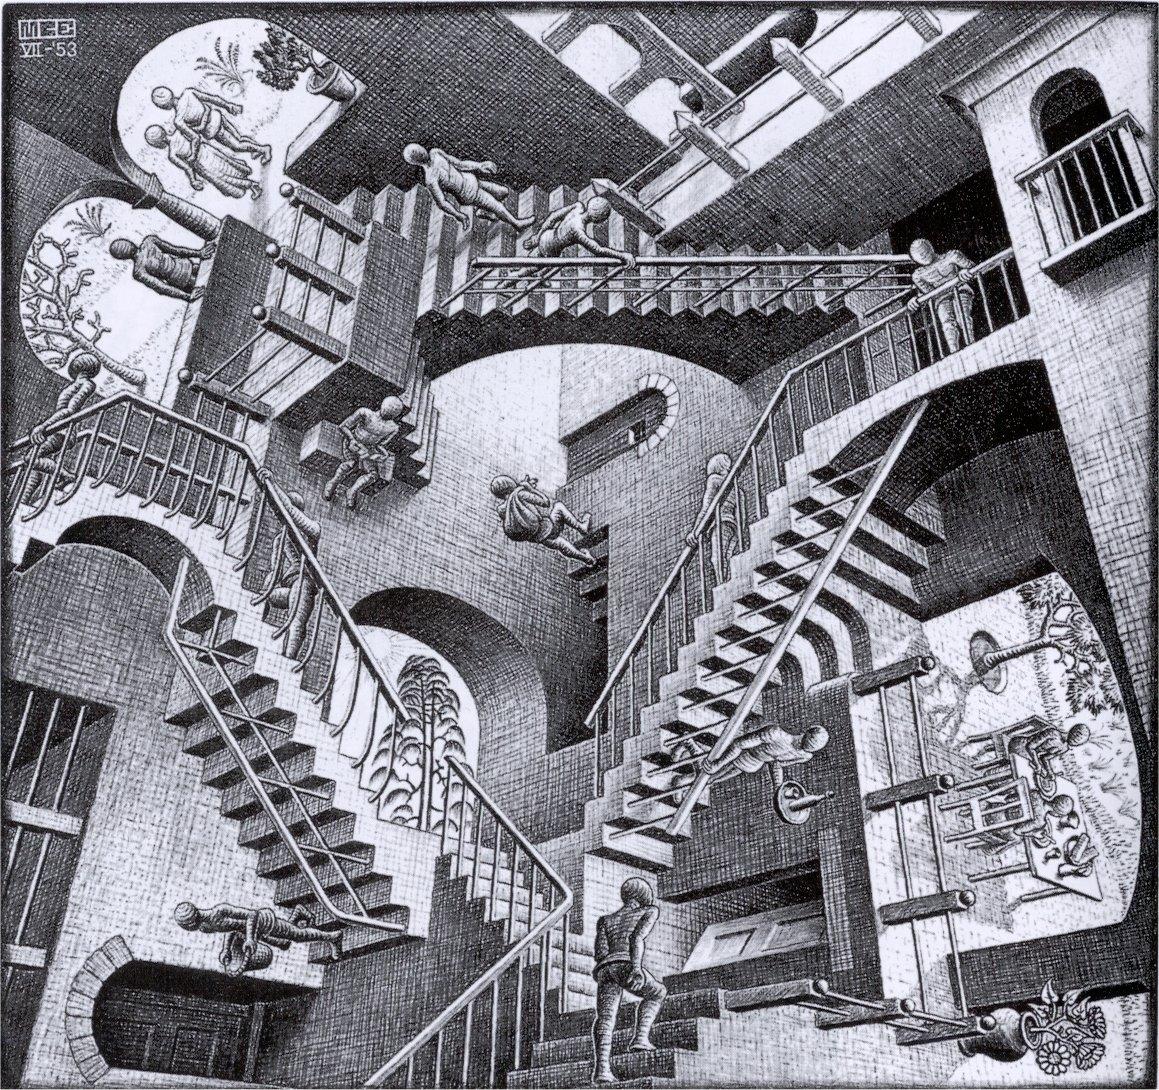
\includegraphics[scale=0.28]{escalerasEscher}

%----------------------------------------------------------------------------------------

\vfill % Fill the rest of the page with whitespace

\end{titlepage}

% ---------------------------------------------------------------------------------------
%         HEADER
%----------------------------------------------------------------------------------------

\fancyhead[L]{Favio Vázquez}
\fancyhead[R]{\thepage}

%----------------------------------------------------------------------------------------
\setcounter{footnote}{0}
\renewcommand*{\thefootnote}{\arabic{footnote}}

\section{Problema 1. Problema 4.1 de Classical Electromagnetic Radiation
de Jackson \cite{jackson}.}

Calcule los momentos multipolares $q_{lm}$ de las distribuciones de carga mostradas 
como las partes $a$ y $b$. Intente obtener resultados para todo los momentos que 
no se hacen cero válidos para todo $l$, pero en cada caso encuentre los primeros 
dos conjuntos de momentos que no se hacen cero al menos.

\begin{figure}[H]
 \center 
 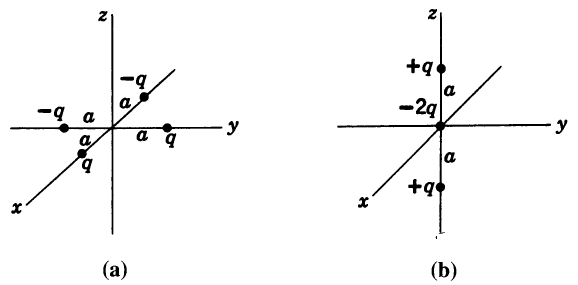
\includegraphics[scale = 0.5]{problema1fig1}
 \caption{Disposición de la distribución de cargas para el problema 1.}
\end{figure}

\begin{enumerate}[label=\textbf{(\alph*)}]
\setcounter{enumi}{2}
\item Para la distribución de carga del segundo conjunto $b$ escriba la expansión 
multipolar para el potencial. Manteniendo solo los términos de orden bajo en la 
expansión, grafique el potencial en el plano $x-y$ como una función de la distancia 
desde el origen para distancias mayores a $a$.
\item Calcule directamente de la ley de Coulomb el potencial exacto para $b$ en 
el plano $x-y$. Grafíquelo como una función de la distancia y compare con el resultados
encontrado en la parte $c$.
\end{enumerate}

Divida la forma asintótica en las partes $c$ y $d$ para ver el comportamiento a 
distancias grandes más claramente.

\vspace{.3cm}

\underline{Solución:} \vspace{.3cm}

Comenzamos recordando la ecuación para los momentos multipolares\footnote{Ver ecuación 
(4.3) de Jackson \cite{jackson}.}

\begin{equation}
 q_{lm} = \sum_i q_ir_i^l Y^*_{lm}(\theta_i,\phi_i),
\end{equation}

donde $(r_i,\theta_i,\phi_i)$ es la posición de la i-ésima carga, $q_i$ es la 
magnitud de la i-ésima carga y $Y^*_{lm}(\theta_i,\phi_i)$ son los armónicos 
esféricos. Viendo la figura de la parte (a) vemos que las cargas, en coordenadas 
esféricas se ubican según la siguiente tabla\footnote{La primera carga es la ubicada 
en $(x=0,y=a,z=0)$}

\begin{table}[H]
\centering
\begin{tabular}{|l|l|l|l|}
\hline
Carga & $r$ & $\theta$ & $\phi$   \\ \hline
$+q$    & $a$ & $\pi/2$  & 0      \\ \hline
$+q$    & $a$ & $\pi/2$  & $\pi/2$  \\ \hline
$-q$    & $a$ & $\pi/2$  & $\pi$    \\ \hline
$-q$    & $a$ & $\pi/2$  & $3\pi/2$ \\ \hline
\end{tabular}
\end{table}

Entonces utilizando esta información tenemos 

\begin{equation}
 q_{lm} = qa^l\left[Y^*_{lm}\left(\frac{\pi}{2},0\right) + 
 Y^*_{lm}\left(\frac{\pi}{2},\frac{\pi}{2}\right) - 
 Y^*_{lm}\left(\frac{\pi}{2},\pi\right) - 
 Y^*_{lm}\left(\frac{\pi}{2},\frac{3\pi}{2}\right)\right].
\end{equation}

Pero recordando que\footnote{Ver ecuación (3.53) y (3.54) de Jackson \cite{jackson}}

\begin{equation}
 Y_{lm}(\theta,\phi) = \sqrt{\frac{2l+1}{4\pi}\frac{(l-m)!}{(l+m)!}}P_l^m(\cos{\theta}) 
 \euler^{im\phi},
 \label{eq:esfericosArmonicosLegendre}
\end{equation}

donde $P_l^m(\cos{\theta}$ son las funciones de Legendre asociadas (ver ecuación 
(3.49) de Jackson) y

\begin{equation}
 Y_{l,-m}(\theta,\phi) = (-1)^m Y^*_{lm}(\theta,\phi), 
\end{equation}

podemos escribir entonces 

\begin{equation*}
 q_{lm} = (-1)^m\sqrt{\frac{2l+1}{4\pi}\frac{(l-m)!}{(l+m)!}} [\euler^{i(-m)(0)} + 
 \euler^{i(-m)(\pi/2)} - \euler^{i(-m)(\pi)} - \euler^{i(-m)(3\pi/2)}] 
 P_l^m(\cancelto{0}{\cos{\frac{\pi}{2}}}),
\end{equation*}

pero 

\begin{align*}
 \euler^{i(-m)(0)} &= 1, \\
 \euler^{i(-m)(\pi/2)} &= (\euler^{-i\pi/2})^{(m)} = (-i)^m, \\
 \euler^{i(-m)(\pi)} &= (\euler^{-i\pi})^{(m)} = (-1)^m, \\
 \euler^{i(-m)(3\pi/2)} &= (\euler^{-i3\pi/2})^{(m)} = i^m.
\end{align*}

Tenemos entonces, 

\begin{equation}
 q_{lm} = qa^l\sqrt{\frac{2l+1}{4\pi}\frac{(l-m)!}{(l+m)!}}\left[1 + 
 (-i)^m - (-1)^m - i^m \right]P_l^m(0),
\end{equation}

el término entre corchetes $\left[1 +  (-i)^m - (-1)^m - i^m \right]$ es cero 
para $m$ par, y se hace $(2-2i)$ para $m = -7,-3,1,5,9,\dots$ y $(2+2i)$ para 
$m=-5,-1,3,7,\dots$, además por las propiedades de $P_l^m(0)$ sabemos que se 
hace cero cuando $l$ y $m$ tienen signos diferentes. Estas dos consideraciones 
no hacen ver que los únicos momentos que no se hacen cero son aquellos con 
$l$ y $m$ impares. Y como el texto lo solicita, los primeros conjuntos de momentos 
que no se hacen cero son 

\begin{equation}
 \boxed{q_{1,\pm 1} = \mp qa\sqrt{\frac{3}{4\pi}} (1 \mp i)},
\end{equation}

\begin{equation}
 \boxed{q_{3,\pm 1} = \pm qa^3\sqrt{\frac{21}{\pi}} (1 \mp i)},
\end{equation}

\begin{equation}
 \boxed{q_{3,\pm 3} = \mp qa^3\sqrt{\frac{35}{16\pi}} (1 \pm i)},
\end{equation}

\newpage

\textbf{(b)} Viendo la figura de la parte (b) vemos que las cargas, en coordenadas 
esféricas se ubican según la siguiente tabla\footnote{La primera carga es la ubicada 
en $(x=0,y=0,z=a)$}

\begin{table}[H]
\centering
\begin{tabular}{|l|l|l|l|}
\hline
Carga 	& $r$ & $\theta$ & $\phi$   \\ \hline
$+q$    & $a$ & $0$ 	 & $0$      \\ \hline
$-2q$   & $0$ & $0$	 & $0$  \\ \hline
$+q$    & $a$ & $\pi$  	 & $0$    \\ \hline
\end{tabular}
\end{table}

Entonces, 

\begin{equation}
 q_{lm} = q\left[a^lY^*_{lm}(0,0) - \cancelto{0}{(0)^l lY^*_{lm}(0,0)} + 
 a^llY^*_{lm}(\pi,0)\right],
\end{equation}

y usando \eqref{eq:esfericosArmonicosLegendre} podemos escribir esto como 

\begin{equation}
 q_{lm} = qa^l\sqrt{\frac{2l+1}{4\pi}\frac{(l-m)!}{(l+m)!}} 
 \left[ e^{im(0)}P_l^m(\cos(0)) + e^{im(0)}P_l^m(\cos(\pi)) \right],
\end{equation}

\begin{equation}
 \therefore q_{lm}qa^l\sqrt{\frac{2l+1}{4\pi}\frac{(l-m)!}{(l+m)!}} 
 \left[P_l^m(1) + P_l^m(-1) \right].
\end{equation}

Debido a que el sistema tiene simetría azimutal, solamente los términos con 
$m=0$ serán distintos de cero, y notando que $P_l^0(1) = 1, P_l^0(-1) = (-1)^l$ 
tenemos que 

\begin{equation}
 q_{l0} = qa^l\left[\frac{2l+1}{4\pi} \right]^{1/2}[1 + (-1)^l],
\end{equation}

y tendremos que para $l$ par y $m=0$, 

\begin{equation}
 q_{l0} = 2qa^l\left[\frac{2l+1}{4\pi} \right],
 \label{eq:momentoCasoB}
\end{equation}

y para $l$ impar o $m \neq 0$ $q_{l0} = 0$. Los primeros momentos que 
no se hacen cero son 

\begin{equation}
 \boxed{q_{2,0} = qa^2\sqrt{\frac{5}{\pi}}},
\end{equation}

\begin{equation}
 \boxed{q_{4,0} = qa^4\sqrt{\frac{9}{\pi}}}.
\end{equation}

\textbf{(c)} La expansión multipolar para el potencial podemos escribirla como\footnote{Ver 
ecuación (4.1) de Jackson \cite{jackson}.} 

\begin{equation}
 \Phi(r,\theta,\phi) = \frac{1}{4\pi\epsilon_0 r}\sum_{l=0}^\infty 
 \sum_{m=-l}^l \frac{4\pi}{2l+1} 
 q_{lm} \frac{Y_{lm}(\theta,\phi)}{r^{l+1}},
\end{equation}

y sustituyendo \eqref{eq:momentoCasoB} obtenemos 

\begin{equation}
 \Phi(r,\theta,\phi) = \frac{1}{4\pi\epsilon_0}\sum_{l=1}^\infty \frac{4\pi}{2l+1}  
 \left(qa^{2l}\sqrt{\frac{(4l+1)}{4\pi}} \right)\frac{Y_{2l,0}(\theta,\phi)}{r^{2l+1}},
\end{equation}

\begin{equation}
 \boxed{\Phi(r,\theta) = \frac{q}{2\pi\epsilon_0 r}\sum_{l=1}P_{2l}(\cos{\theta})
 \left(\frac{a}{r}\right)^{2l}}.
\end{equation}

El término de orden más bajo se da cuando $l=1$, 

\begin{equation}
 \Phi(r,\theta) = \frac{q}{4\pi\epsilon_0}\frac{a^2}{r^3}\left[ 
 \frac{1}{2}(3\cos^2{\theta} - 1)\right],
\end{equation}

que en el plano $x-y$, donde $\theta = \pi/2$ tenemos 

\begin{equation}
 \Phi_{x-y}(r,\theta) = - \frac{q}{8\pi\epsilon_0}\frac{a^2}{r^3}.
\end{equation}

Cuyo gráfico es 

\begin{figure}[H]
\center 
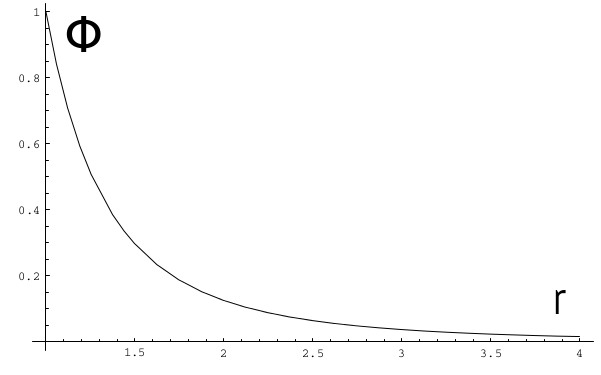
\includegraphics[scale=0.6]{problema1fig2}
\caption{Gráfico del potencial aproximado utilizando expansión multipolar 
para términos de orden bajo en el plano $x-y$.}
\end{figure}

\textbf{(d)} Utilizando la ley de Coulomb podemos escribir el potencial como

\begin{align*}
 \Phi = \frac{1}{4\pi\epsilon_0}\left[\frac{1}{|\mathbf{r} + a\hat{\mathbf{z}}|}
 \frac{1}{|\mathbf{r} - a\hat{\mathbf{z}}|} - \frac{2}{|\mathbf{r}|} \right],
\end{align*}

que en el plano $x-y$ se escribe 

\begin{equation}
 \Phi = \frac{2q}{4\pi\epsilon_0}\left[\frac{1}{\sqrt{r^2+a^2}} - \frac{1}{r} \right],
\end{equation}

o 

\begin{equation}
 \boxed{\Phi = \frac{q}{4\pi\epsilon_0 a}\left[\frac{2}{\sqrt{(r/a)^2 + 1}} - 
 \frac{2}{(r/a)}\right]}.
\end{equation}

\newpage

Cuyo gráfico es 

\begin{figure}[H]
\center 
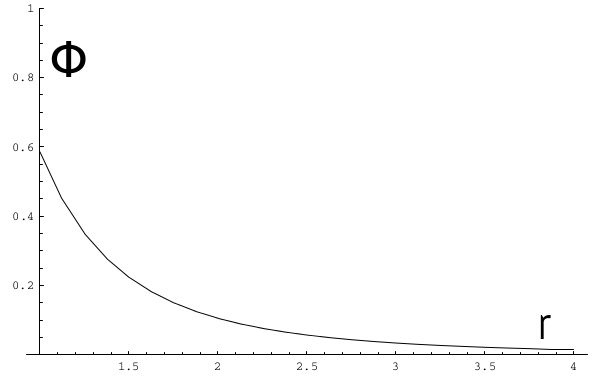
\includegraphics[scale=0.6]{problema1fig3}
\caption{Gráfico del potencial exacto, en el plano $x-y$,
utilizando la ley de Coulomb}
\end{figure}

Con lo cual vemos que el primer término en la expansión multipolar es una buena 
aproximación para distancias $r \approx 2a$, pero impreciso para otras más pequeñas.

\vspace{.3cm}

Si dividimos ahora la forma asintótica en las partes (c) y (d) para ver el comportamiento 
a distancias grandes, lo que tenemos que hacer es dividir por $1/r^3$ tanto 
el potencial aproximado como el exacto, obteniendo el siguiente gráfico

\begin{figure}[H]
\center 
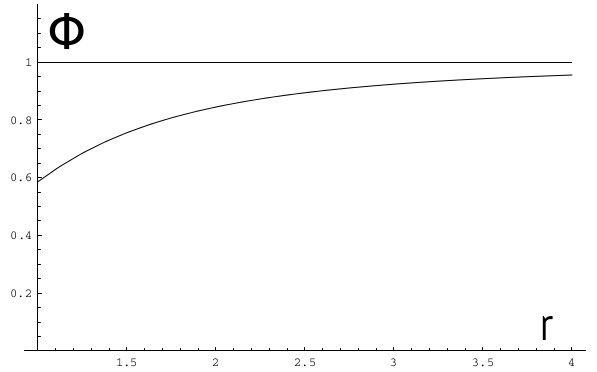
\includegraphics[scale=0.6]{problema1fig4}
\caption{Comportamiento del potencial tanto para la forma aproximada como para 
la exacta, donde se ha dividido la forma asintótica. La línea recta es la aproximación 
de la parte (c) y la otra es la obtenida con la ley de Coulomb en la parte (d).}
\end{figure}

Vemos que la aproximación mejora para $r \gg a$. 

\newpage

\section{Problema 2. Problema 4.7 de Classical Electromagnetic Radiation
de Jackson \cite{jackson}.}

Una distribución de carga localizada tiene la densidad de carga 

$$
\rho(\mathbf{r}) = \frac{1}{64\pi}r^2\euler^{-r}\sen^2{\theta}
$$

\begin{enumerate}[label=\textbf{(\alph*)}]
\item Haga una expansión multipolar del potencial debido a esta densidad de 
carga y determine todos los momentos multipolares que no se hacen cero. Escriba 
el potencial a grandes distancias como una expansión finita en polinomios de 
Legendre. 
\item Determine el potencial explícitamente en cualquier punto del espacio, y 
muestre que cerca del origen, correcto a $r^2$ inclusive,

$$
\Phi(\mathbf{r}) \simeq \frac{1}{4\pi\epsilon_0}\left[\frac{1}{4} 
 - \frac{r^2}{120}P_2(\cos{\theta})\right]
$$

\item Si existe en el origen un núcleo con un momento cuadrupolar $Q = 10^{-28}$ m$^2$, 
determine la magnitud de la energía de interacción, asumiendo que la unidad de 
carga en $\rho(\mathbf{r})$ arriba es la carga electrónica y que la unidad de 
longitud es el radio de Bohr del hidrógeno $a_0 = 4\pi\epsilon_0\hslash/me^2 = 
0.529 \times 10^{-10}$ m. Exprese su respuesta como una frecuencia dividida por 
la constante de Planck $h$.
\end{enumerate}

La densidad de carga en este problema es la de los estados $m = \pm 1$ del nivel 
$2p$ en el hidrógeno, mientras que la interacción cuadrupolar es del mismo orden 
que el encontrado en moléculas.

\vspace{.3cm}

\underline{Solución:} \vspace{.3cm}

\newpage

\section{Problema 3. Problema 4.8 de Classical Electromagnetic Radiation
de Jackson \cite{jackson}.}

Un cascarón cilíndrico, muy largo y circular recto, de constante dieléctrica 
$\epsilon/\epsilon_0$ y radio interno y externo $a$ y $b$, respectivamente, 
es colocado en un previamente campo eléctrico uniforme $E_0$ con su eje perpendicular 
al campo. El medio adentro y afuera del cilindro tiene una constante dieléctrica de 
uno.

\begin{enumerate}[label=\textbf{(\alph*)}]
\item Determine el potencial y campo eléctrico en las tres regiones, despreciando 
efectos finales.
\item Esboce las líneas de fuerza para un caso típico de $b \simeq 2a$.
\item Discuta las formas limitantes en su solución apropiadas para un cilindro 
dieléctrico sólido en un campo uniforme, y una cavidad cilíndrica en un dieléctrico 
uniforme.
\end{enumerate}

\vspace{.3cm}

\underline{Solución:} \vspace{.3cm}

\newpage

\section{Problema 4. Problema 4.9 de Classical Electromagnetic Radiation
de Jackson \cite{jackson}.}

Una carga puntual $q$ es colocada en el espacio libre a una distancia $d$ del centro 
de una esfera dieléctrica de radio $a$ ($a < d)$ y constante dieléctrica 
$\epsilon/\epsilon_0$. 

\begin{enumerate}[label=\textbf{(\alph*)}]
\item Encuentre el potencial en todos los puntos del espacio como una expansión 
en armónicos esféricos.
\item Calcule las componentes rectangulares del campo eléctrico cerca del 
centro de la esfera.
\item Verifique que, en el límite $\epsilon/\epsilon_0 \rightarrow \infty$, tu 
resultado es el mismo que para la esfera conductora.
\end{enumerate}

\vspace{.3cm}

\underline{Solución:} \vspace{.3cm}

\newpage

\section{Problema 5. Problema 4.13 de Classical Electromagnetic Radiation
de Jackson \cite{jackson}.}

Dos superficies cilíndricas conductoras, largas y coaxiales, de radios $a$ y $b$ 
son bajadas verticalmente a un líquido dieléctrico. Si el líquido sube una altura 
promedio de $h$ entre los electrodos cuando una diferencia de potencial $V$ es 
establecida entre ellos, muestre que la susceptibilidad del líquido es 

$$
\chi_e = \frac{(b^2 - a^2)\rho g h \ln{(b/a)}}{\epsilon_0 V^2}
$$

donde $\rho$ es la densidad del líquido, $g$ es la aceleración debida a la gravedad, 
y la susceptibilidad del aire es depreciada.

\vspace{.3cm}

\underline{Solución:} \vspace{.3cm}

\newpage

\begin{thebibliography}{10}
\bibitem{jackson}
J. Jackson, \emph{Classical Electrodynamics}, 3ra edición. John Wiley and Sons, Inc. 
1999.
\end{thebibliography}

\end{document}